\documentclass{exam}

\usepackage{amsmath,amssymb,amsfonts,amsthm,dsfont}
\usepackage{lib/extra}
\usepackage{graphicx}
\usepackage{tikz}
\usepackage{enumitem}
\usepackage{bbm}
\usepackage{pgfplots}
\usepackage{fontenc}
\usepackage{float}

\pgfplotsset{compat=1.18}

\title{Complex Analysis Chapter 1 Section 1}
\author{Brandyn Tucknott}
\date{Last Updated: 24 September 2025}

\begin{document}
\maketitle

\section{Complex Numbers and the Complex Plane}
\subsection{Basic Properties}
A complex number is of form $z = x + iy$ where $x,y$ are real numbers and $i$ is imaginary
satifying $i^2 = -1$. We call $x$ the \textbf{real part} and $y$ the \textbf{imaginary part} 
of $z$. We write this as 
$$x = \re{z} \qquad \text{ and } \qquad y = \im{z}.$$

We also take note that real numbers are complex numbers with zero imaginary parts, and we call a 
complex number with zero real parts \textbf{purely imaginary}. We can visualize the complex plane
by identifying any complex number $z = x + iy$ with the point $(x, y)$ in the Euclidean plane. We
call the $x$-axis the \textbf{real axis} and the $y$-axis the \textbf{imaginary axis} (see Figure 1).

\begin{figure}[H]
    \centering
    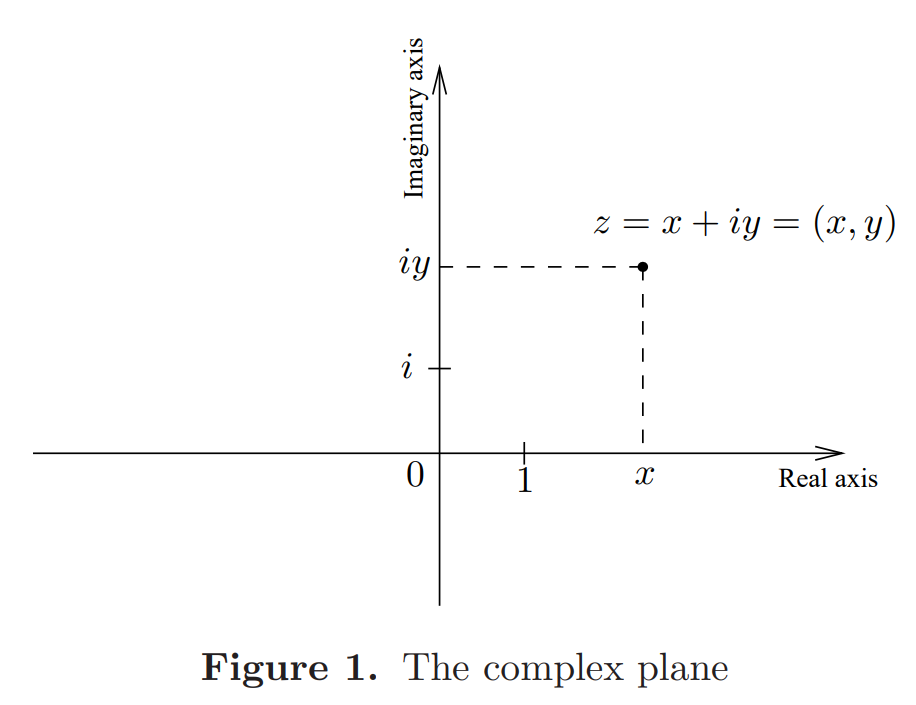
\includegraphics[width=0.5\textwidth]{figures/complex_analysis/figure_1.png}
    % \caption{The complex plane}
\end{figure}

The rules for adding and multiplying complex numbers can all be obtained by treating all numbers as
real numbers, noting that $i^2 = -1$. Below we show both rules and their derivations.
\begin{align*}
    z_1 + z_2 &= (x_1 + iy_1) + (x_2 + iy_2) \\
    &= x_1 + x_2 + iy_1 + iy_2 \\
    &= (x_1 + x_2) + i(y_1 + y_2)
\end{align*}

\begin{align*}
    z_1 z_2 &= (x_1 + iy_1)(x_2 + iy_2) \\
    &= x_1x_2 + x_1iy_2 + iy_1x_2 + i^2y_1y_2 \\
    &= (x_1x_2 - y_1y_2) + i(x_1y_2 + x_2y_1)
\end{align*}

\newpage

Using the two definitions above, we can verify that commutativity, associativity, and distributivity
hold for complex numbers.

\begin{align*}
    \text{Commutativity: }z_1 + z_2 &= (x_1 + x_2) + i(y_1 + y_2) \\
    &= (x_2 + x_1) + i(y_2 + y_1) \\
    &= z_2 + z_1
\end{align*}

\begin{align*}
    \text{Associativity: }(z_1 + z_2) + z_3 &= ((x_1 + x_2) + i(y_1 + y_2)) + (x_3 + iy_3) \\
    &= x_1 + x_2 + x_3 + iy_1 + iy_2 + iy_3 \\
    &= x_1 + iy_1 + (x_2 + x_3) + i(y_2 + y_3) \\
    &= z_1 + (z_2 + z_3)
\end{align*}

\begin{align*}
    \text{Distributivity: }z_1(z_2 + z_3) &= (x_1 + iy_1)((x_2 + x_3) + i(y_2 + y_3)) \\
    &= (x_1 + iy_1)(x_2 + x_3) + (x_1 + iy_1)i(y_2 + y_3) \\
    &= x_1x_2 + x_1x_3 + iy_1x_2 + iy_1x_3 + x_1iy_2 + x_1iy_3 + i^2y_1y_2 + i^2y_1y_3 \\
    &= (x_1x_2 - y_1y_2) + i(y_1x_2 + y_2x_1) + (x_1x_3 - y_1y_3) + i(y_1x_3 + y_3x_1) \\
    &= z_1z_2 + z_1z_3
\end{align*}

An astute reader may have noticed that addition and multiplication of complex numbers corresponds
with vector addition and dilated rotation. This fact will become more apparent when we introduce
the polar form of a complex number, but for now note that multiplication by $i$ corresponds
to a rotation by an angle of $\frac{\pi}{2}$.

The notion of length or \textbf{absolute value} is still the same, and thinking of complex numbers as vectors
for this purpose makes it easy to define the aboslute value (distance from the origin) of a
complex number:
$$|z| = \sqrt{x^2 + y^2}.$$

Here, we list some useful inequalities that hold for complex numbers. Let $\C$ denote the set of
all complex numbers. Then for all $z, w \in \C$, we have the following:
\begin{itemize}
    \item $|z + w| \leq |z| + |w|$ (Triangle Inequality)
    \item $|\re{z}| \leq |z|$ and $|\im{z}| \leq |z|$
    \item $||z| - |w|| \leq |z - w|$ (Reverse Triangle Inequality)
\end{itemize}


We define the \textbf{complex conjugate} of $z = x + iy$ to be the point reflected across the real
axis in the complex plane.
$$\overline{z} = x - iy.$$

A complex is real if and only if $z = \overline{z}$, and purely imaginary if and only if
$z = -\overline{z}$. 

By directly using the definitions of complex numbers and their conjugates, we can verify that
$$\re{z} = \frac{z + \overline{z}}{2}\qquad \text{ and } \qquad \im{z} = \frac{z - \overline{z}}{2i}$$
and also that
$$|z|^2 = z\overline{z} \longrightarrow \frac{1}{z} = \frac{\overline{z}}{|z|^2} \text{ whenever } z \neq 0$$

\newpage

We now introduce the \textbf{polar form} of a complex number. Any non-zero complex number can be written as
$$z = re^{i\theta}$$
where $r > 0$ and $\theta \in \R$. Here, $\theta$ is often called the \textbf{argument} of $z$, is
defined uniquely up to a multiple of $2\pi$, and is denoted by $\arg{z}$.

Another important definition,
$$e^{i\theta} = \cos{\theta} + i\sin{\theta}$$
and since $\abs{e^{i\theta}} = 1$, we see that $r = |z|$ with $\theta$ as the angle (with positive
counter clockwise orientation) between the real axis and the line segment from the origin to $z$.

\begin{figure}[H]
    \centering
    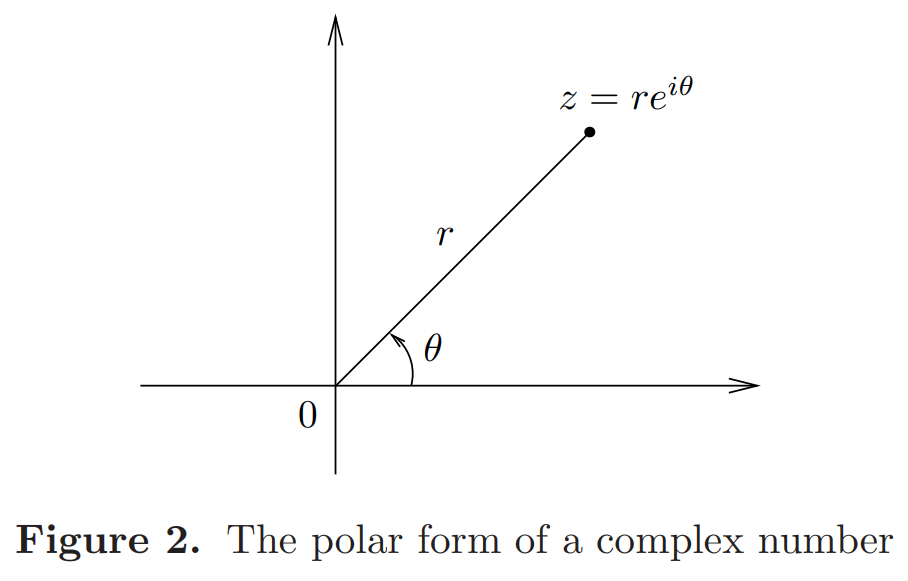
\includegraphics[width=0.5\textwidth]{figures/complex_analysis/figure_2.png}
\end{figure}

Finally, note that if $z = re^{i\theta}$ and $w = se^{i\phi}$, then
$$zw = rse^{i(\theta + \phi)},$$
which allows us to plainly see why multiplication of complex numbers corresponds to
dilated rotation in $\R^2$.

\subsection{Convergence}
A sequence of complex numbers $\cbrac{z_1, z_2, \hdots}$ is said to \textbf{converge} to $w\in\C$
$$\lim_{n\to\infty} \abs{z_n - w} = 0, \quad \text{ and we write } w = \lim_{n\to\infty} z_n.$$

It is also true that a sequence $\cbrac{z_n}$ converges to $w$ if and only if the
real and imaginary parts of $\cbrac{z_n}$ converge to the real and imaginary parts of $w$ respectively.
Since it is sometimes not possible to readily identify the limit of a sequence, we have a condition
on the sequence itself which is equivalent to convergence. A  sequence $\cbrac{z_n}$ is said to be
a \textbf{Cauchy Sequence} (or just \textbf{Cauchy}) if
$$\abs{z_n - z_m} \rightarrow 0 \text{ as } n,m\to\infty.$$

More definitively, given $\veps > 0$ there exists an integer $N > 0$ such that $\abs{z_n - z_m} < \veps$
whenever $n,m > N$. Since $\R$ is complete, every Cauchy sequence of real numbers converges
to a real number, and since a squence is Cauchy if and only if itselfs real and imaginary parts are Cauchy,
we have that every Cauchy sequence in $\C$ has a limit in $\C$. This brings us to our first theorem.

\begin{theorem}\label{thm:main}
    $\C$ is complete.
\end{theorem}


\subsection{Sets in the Complex Plane}
Below we list some common sets. Let $z_0\in\C$ and $r > 0$.
\begin{itemize}
    \item \textbf{Open Disk of radius }$r$\textbf{ centered at }$z_0$
    $$D_r(z_0) = \cbrac{z\in\C : \abs{z - z_0} < r}$$
    \item \textbf{Closed Disk of radius }$r$\textbf{ centered at }$z_0$
    $$\overline{D_r}(z_0) = \cbrac{z\in\C : \abs{z - z_0} \leq r}$$
    \item \textbf{Boundary of a Disk}$r$\textbf{ centered at }$z_0$
    $$C_r(z_0) = \cbrac{z\in\C : \abs{z - z_0} = r}$$
    \item \textbf{Unit Disk}  (Radius 1 centered at the origin)
    $$\mathbb{D} = \cbrac{z\in\C : \abs{z} < 1}$$
\end{itemize}

We follow up with some definitions for these (or really any) sets. Given a set $\Omega\subset\C$,
a point $z_0\in\C$ is an \textbf{interior point} fo $\Omega$ if there exists $r > 0$ such that 
$D_r(z_0) \subset\Omega$. The \textbf{interior} of $\Omega$ consists of all interior points. We 
call $\Omega$ \textbf{open} if every point in $\Omega$ is an interior point. $\Omega$ is \textbf{closed} if
its complement $\Omega^c = \C - \Omega$ is open.

Equivalently, a point $z\in\C$ is said to be a \textbf{limit point} of $\Omega$ if there exists
a sequence of points $z_n\in\C$ such that $z_n \neq z$ and $\lim_{n\to\infty} z_n = z$. With this,
we can check that a set is closed if and only if it contains all of its limit points. The \textbf{closure}
of any set $\Omega$ is the union of $\Omega$ and its limit points, and is denoted by $\overline{\Omega}$.

Finally, the \textbf{boundary} of a set $\Omega$ is equal to its closure minus its interior, and is denoted
by $\partial \Omega$. A set is bounded if there exists $M > 0$ such that $\abs{z} < M$ for all
$z\in M$ (intuitively, if $\Omega$ is contained by some disk). If $\Omega$ is bounded, its \textbf{diameter} 
is defined to be
$$\text{diam}(\Omega) = \sup_{z,w\in \Omega} \abs{z - w}.$$

A set $\Omega$ is said to be \textbf{compact} if it is closed and bounded.


\begin{theorem}\label{thm:main}
    The set $\Omega\subset\C$ is compact if and only if every sequence of $\cbrac{z_n}\subset \Omega$
    has a subsequence that converges to a point in $\Omega$.
\end{theorem}

An open covering of $\Omega$ is a family of (not necessarily countable) open sets $\cbrac{U_\alpha}$
such that
$$\Omega \subset \bigcup_\alpha U_\alpha.$$

\begin{theorem}\label{thm:main}
    The set $\Omega\subset\C$ is compact if and only if every open covering of $\Omega$ has a finite
    subcovering.
\end{theorem}

\begin{proposition}\label{prop:main}
    If $\Omega_1 \supset \Omega_2 \supset \hdots \supset \Omega_n \supset \hdots$ is a sequence of 
    non-empty compact sets in $\C$ with the property that
    $$\text{diam}\paren{\Omega_n} \to 0 \text{ as } n\to\infty,$$
    then there exists a unique point $w\in\C$ such that $w\in\Omega_n$ for all $n$.
\end{proposition}
\begin{proof}
    Choose a point $z_n$ in each $\Omega_n$. The condition diam$(\Omega_n)\to 0$ implies that $\cbrac{z_n}$
    is Cauchy, and therefore converges to some limit which we call $w$. Since each set $\Omega_n$ is
    compact, we must have $w\in\Omega_n$ for all $n$. Finally, $w$ is the unique point satisfying
    this property. If there were some other $w'$ satisfying the same property with $w' \neq w$, then 
    $\abs{w - w'} > 0$ and the condition diam$(\Omega_n)$ would be violated.
\end{proof}

An open set $\Omega$ is said to be \textbf{connected} if it is not possible to find two disjoint 
non-empty open set $\Omega_1, \Omega_2$ such that
$$\Omega = \Omega_1 \cup \Omega_2.$$
A connected open set in $\C$ will be called a \textbf{region}. A similar notion of connectivity is 
true for closed sets.

Another similar, very pratical definition for connected open sets: an open set $\Omega$ is connected
if and only if any two points in $\Omega$ can be joined by a curve $\gamma$ entirely contained in $\Omega$. 

\end{document}